\documentclass[c]{beamer}

\usetheme{default}
\usefonttheme{structurebold}

\usepackage[utf8]{inputenc}
\usepackage{lmodern}

\usepackage[]{amsmath}
\usepackage{amsfonts}

\usepackage{graphicx}

\author{Igor Colin}
\date{\today}

\begin{document}

\begin{frame}
    \frametitle{Principe de l'application}

    \begin{itemize}
        \item Partage entre utilisateurs
            \begin{itemize}
                \item texte
                \item image
                \item vidéo
                \item géolocalisation
                \item fichier
            \end{itemize}
        \item Recommandations d'événements
            \begin{itemize}
                \item personnalisées
                \item possibilité de faire suivre à d'autres utilisateurs
            \end{itemize}
        \item Objectif
            \begin{itemize}
                \item modéliser les échanges d'informations
                \item établir profils et liens entre utilisateurs
                \item faire des recommandations personnalisées
            \end{itemize}
    \end{itemize}
\end{frame}

\begin{frame}
    \frametitle{Graphes}

    \begin{columns}
        \begin{column}{.5\textwidth}
            \begin{itemize}
                \item<1-> Graphe $G = (V,E)$
                \item<2-> N\oe{}uds $V = \{v_1,\ldots,v_n\}$
                \item<3-> Arrêtes $E = \{e_1,\ldots,e_m\}$
                    \begin{itemize}
                        \item<4-> $e = (u,v) \in V \times V$
                        \item<5-> $e = \{(u,v), (v,u)\}$
                        \item<6-> $e = (u,v,l) \in V \times V \times L$
                    \end{itemize}
            \end{itemize}
        \end{column}
        \begin{column}{.5\textwidth}
            \only<2>{
                \begin{figure}
                    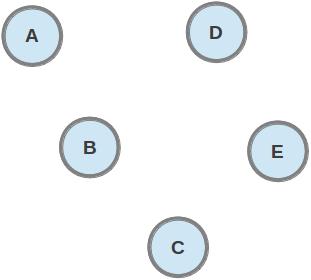
\includegraphics[width=.7\textwidth]{./figures/utilisateurs.png}
                \end{figure}
            }
            \only<3>{
                \begin{figure}
                    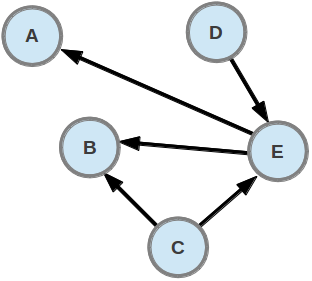
\includegraphics[width=.7\textwidth]{./figures/arretes.png}
                \end{figure}
            }
            \only<4>{
                \begin{figure}
                    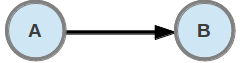
\includegraphics[width=.7\textwidth]{./figures/arretes_orientees.png}
                \end{figure}
            }
            \only<5>{
                \begin{figure}
                    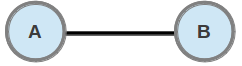
\includegraphics[width=.7\textwidth]{./figures/arretes_non-orientees.png}
                \end{figure}
            }
            \only<6>{
                \begin{figure}
                    
\includegraphics[width=.7\textwidth]{./figures/arretes_etiquettes.png}
                \end{figure}
            }

        \end{column}
    \end{columns}

\end{frame}

\begin{frame}
    \frametitle{Statistiques}

    \begin{columns}
        \begin{column}{.6\textwidth}
            \begin{itemize}
                \item<1-> Degré :
                    \begin{itemize}
                        \item entrant, sortant
                        \item moyenne, minimum, maximum
                        \item distribution (loi puissance)
                    \end{itemize}
                \item<2-> Diamètre
                    \begin{itemize}
                        \item réel
                        \item efficace
                    \end{itemize}
                \item<3-> Conductance / expansion
                \item<4-> Matrice d'adjacence, matrice laplacienne
            \end{itemize}
        \end{column}
        \begin{column}{.4\textwidth}
            \only<1>{
                \begin{figure}
                    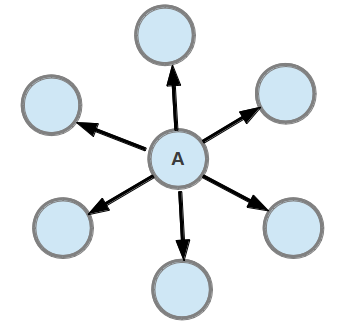
\includegraphics[width=.7\textwidth]{./figures/degre_in-out.png}
                \end{figure}
                \begin{figure}
                    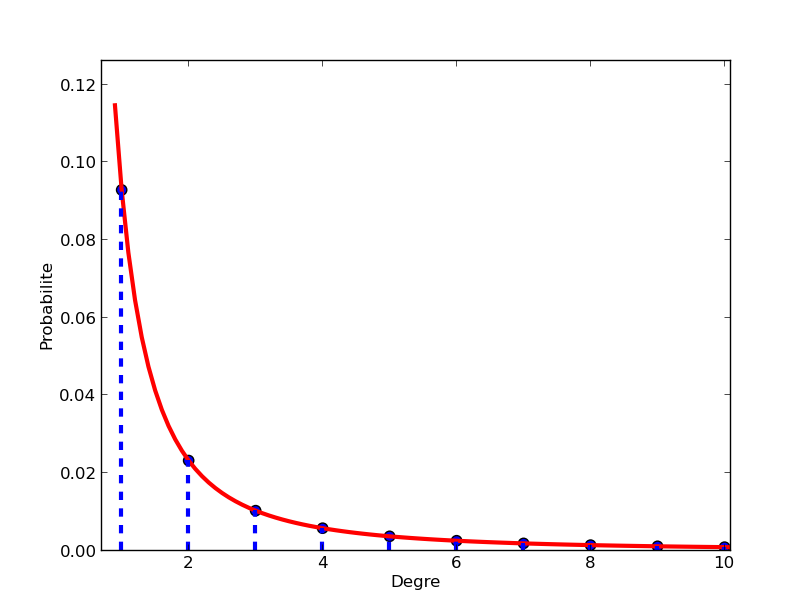
\includegraphics[width=.9\textwidth]{./figures/degre_power-law.png}
                \end{figure}
            }
            \only<2->{
                \begin{figure}
                    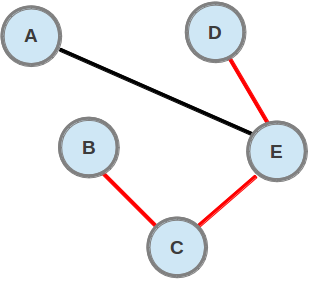
\includegraphics[width=.7\textwidth]{./figures/diametre.png}
                \end{figure}
            }
        \end{column}
    \end{columns}
\end{frame}

\begin{frame}
    \frametitle{Génération de graphes}

    \begin{itemize}
        \item<1-> Objectif : pouvoir générer des graphes aux propriétés similaires
        \item<2-> Méthodes
            \begin{itemize}
                \item Attachement préférentiel (Newman), Fitness model : 
                    \begin{itemize}
                        \item lorsqu'un réseau grandit, les nouveaux n\oe{}uds
                            ne se connectent pas aléatoirement
                        \item ils se connectent aux n\oe{}uds les plus attirants
                    \end{itemize}
                \item Kronecker (Leskovec)
            \end{itemize}
        \item<3-> Optimiser les paramètres des modèles pour obtenir des graphes
            aux propriétés similaires.
    \end{itemize}
\end{frame}

\begin{frame}
    \frametitle{Détection de communautés}

    \begin{columns}
        \begin{column}{.7\textwidth}
            \begin{itemize}
                \item<1-> Idée :
                    \begin{itemize}
                        \item Un graphe peu contenir des sous-graphes très connectés
                        \item Deux utilisateurs d'un même sous-graphe peuvent avoir un profil
                            similaire
                    \end{itemize}
                \item<2-> Méthode :
                    \begin{itemize}
                        \item Sélection d'un critère de qualité de partionnement (modularité)
                        \item Sélection des deux sous-graphes maximisant le critère
                        \item Itération sur les sous-graphes jusqu'à ce que le critère n'augmente plus
                    \end{itemize}
                \item<3-> Graphe \textit{monolabel} (Newman 2006)
                \item<4-> Graphe \textit{multilabel} (Lelarge, Massoulié, Xu 2013)
            \end{itemize}
        \end{column}
        \begin{column}{.3\textwidth}
            \begin{figure}
                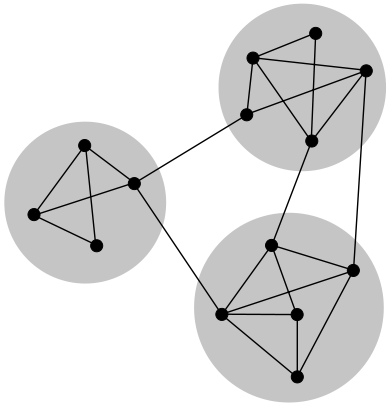
\includegraphics[width=.9\textwidth]{./figures/detection_communaute.png}
            \end{figure}
        \end{column}
    \end{columns}
\end{frame}

\begin{frame}
    \frametitle{Propagation de l'information}

    \begin{itemize}
        \item<1-> Détection de communauté : structure du graphe
        \item<2-> Modéliser la propagation de l'information
            \begin{itemize}
                \item Théorie de la survie
                \item Influences dans un réseau, théorie de la percolation
            \end{itemize}
    \end{itemize}
\end{frame}

\begin{frame}
    \frametitle{Autres problèmes}

    \begin{itemize}
        \item<1-> Statique vs dynamique :
            \begin{itemize}
                \item Beaucoup de modèles/méthodes basées sur des graphes statiques
                \item En réalité, $G(t) = (V(t), E(t))$
                \item Nécessité de méthodes adaptées (online)
            \end{itemize}
        \item<2-> Parcimonie des recommandations :
            \begin{itemize}
                \item Beaucoup de possibilités de recommandations
                \item Ne pas submerger de recommandations
                \item Introduction d'une pénalité
            \end{itemize}
    \end{itemize}
\end{frame}

\end{document}
